\textbf{8-1.}在如习题 8-1 图所示的装置中, 已知容器与容器内液体的总质量为 $5.0 \mathrm{~kg}$ , 吊在弹簧秤下的重物是边长为 $8.0 \mathrm{~cm}$ 的立方体, 弹簧秤的读数为 $6.0 \mathrm{~kg}$ , 台秤的读数为 $8.1 \mathrm{~kg}$ 。求: 

(1) 重物的质量; 

(2) 容器内液体的密度。

\begin{figure}[H]
  \centering
  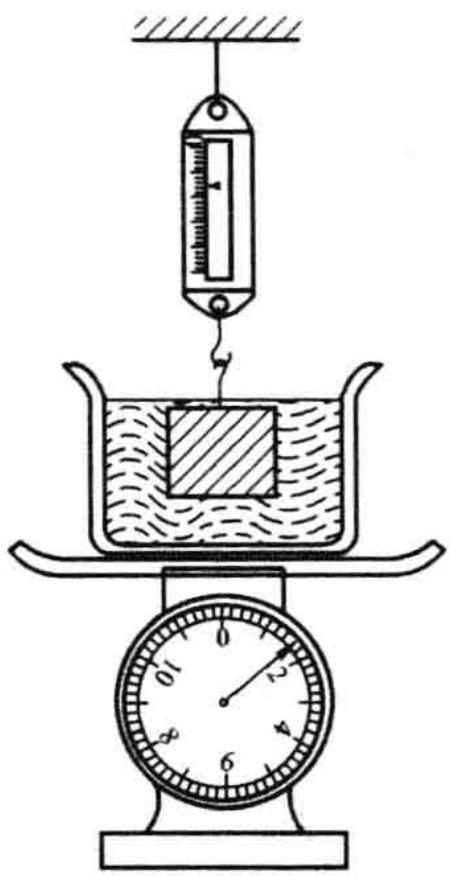
\includegraphics[width=0.15\textwidth]{figures/fig8-1.jpg}
  \end{figure}

\vfill

\textbf{8-2.}一根横截面积 $S_{1} = 5.00 \mathrm{~cm}^{2}$ 的细管, 连接在一个容器上, 容器的横截面积 $S_{2} = 100 \mathrm{~cm}^{2}$ , 高度 $h_{2} = 5.00 \mathrm{~cm}$ 。把水注入, 使水至容器底部的高度 $h_{1} + h_{2} = 100 \mathrm{~cm}$ , 如习题 8-2 图所示。求:

(1) 水对容器底部的作用力为多大?

(2) 此装置内水的重力为多大?

(3) 解释(1)、(2)所求得的结果为何不同?

\begin{figure}[H]
  \centering
  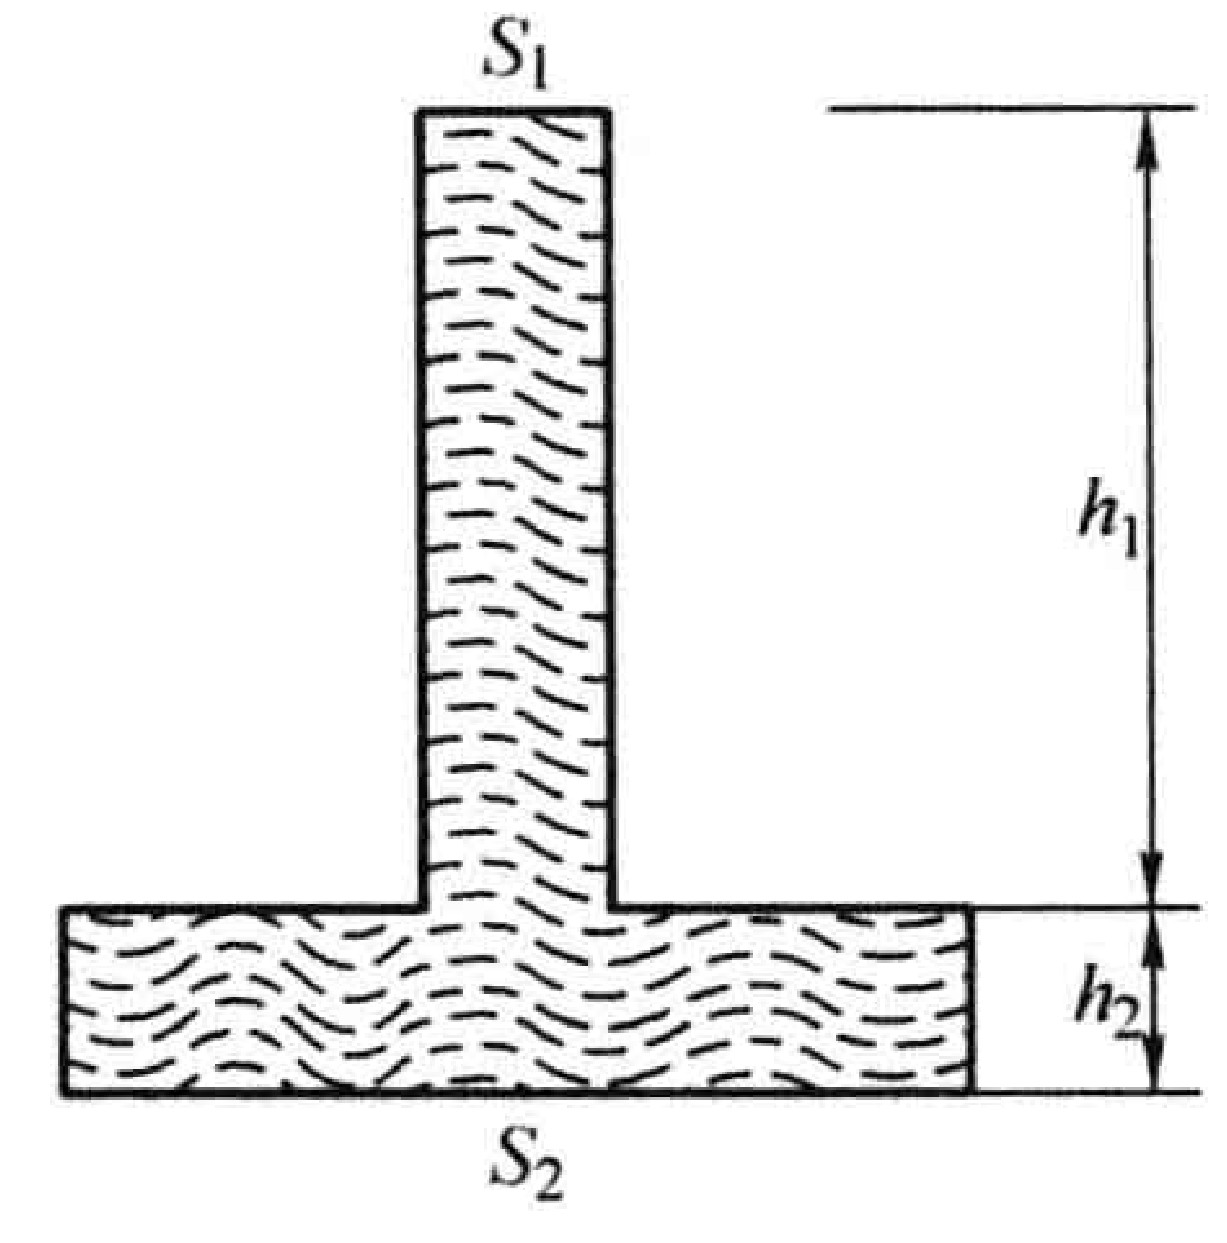
\includegraphics[width=0.25\textwidth]{figures/fig8-2.jpg}
  \end{figure}

\vfill
\newpage

\textbf{8-3.}一根长为 $l$ 、密度为 $\rho$ 的均质细杆, 浮在密度为 $\rho_{0}$ 的液体里。杆的一端由一竖直细绳悬挂着,使该端高出液面的距离为d,如习题8-3图所示。试求:(1)杆与液面的夹角 $\theta$ ;(2)绳中的张力 $F_{T}$ 。设杆的横截面积为S。

\begin{figure}[H]
  \centering
  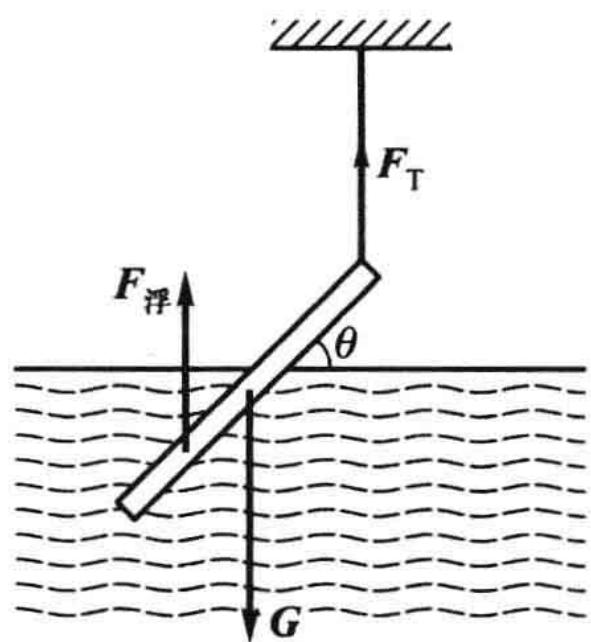
\includegraphics[width=0.25\textwidth]{figures/fig8-3.jpg}
  \end{figure}

\vfill

\textbf{8-4.}若上题中细杆的一端由一竖直细绳与装液体的容器底面相连, 使该端低于液面的距离为 $d$ , 如习题 8-4 图所示。求解上题中的两个问题。

\begin{figure}[H]
  \centering
  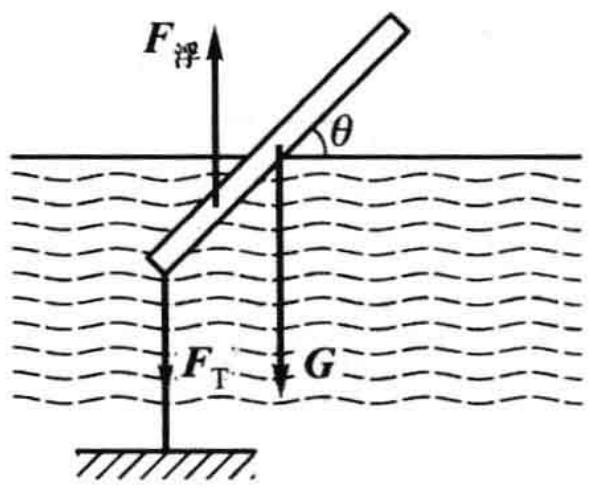
\includegraphics[width=0.25\textwidth]{figures/fig8-4.jpg}
  \end{figure}

\vfill
\newpage

\textbf{8-5.}一粗细均匀的 U 形管内装有一定量的液体。U 形管底部的长度为 $l$ 。当 U 形管以加速度 $a$ 沿水平方向加速时, 如习题 8-5 图所示, 求两管内液面的高度差 $h$ 。
\begin{figure}[H]
  \centering
  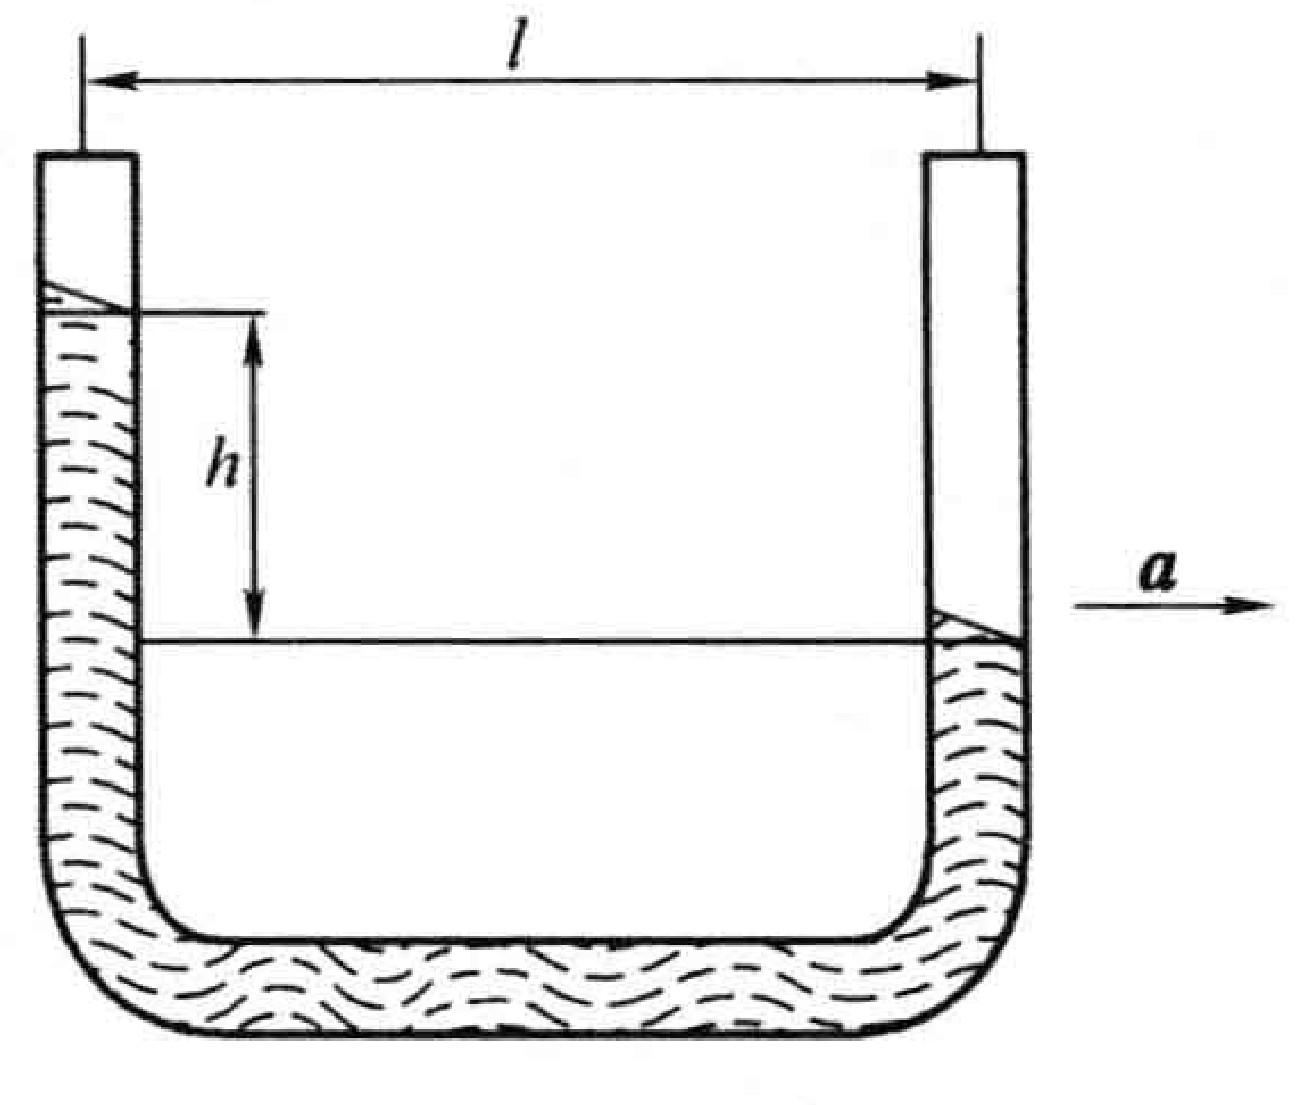
\includegraphics[width=0.25\textwidth]{figures/fig8-5.jpg}
  \end{figure}

\vfill

\textbf{8-6.}一立方体钢块平正地浮在容器内的水银中。已知钢块的密度为 $7.8 \mathrm{~g} / \mathrm{cm}^{3}$ , 水银的密度为 $13.6 \mathrm{~g} / \mathrm{cm}^{3}$ 。

(1) 问钢块露出水银面之上的高度与边长之比为多大?

(2) 如果在水银面上加水,使水面恰与钢块的顶相平,问水层的厚度与钢块边长的比例为多大?

\vfill
\newpage

\textbf{8-7.}利用一根跨过水坝的粗细均匀的虹吸管,从水库里取水,如习题 8-7 图所示,已知水库的水位的深度 $h_A = 2.00 \mathrm{~m}$ , 虹吸管出水口的高度 $h_B = 1.00 \mathrm{~m}$ , 坝高 $h_C = 2.50 \mathrm{~m}$ 。设水在虹吸管内做定常流动。

(1) 求 A、B、C 三个位置处的压强；

(2) 若虹吸管的横截面积为 $7.00 \times 10^{-4} \mathrm{~m}^{2}$ , 求水从虹吸管流出的体积流量。

\begin{figure}[H]
  \centering
  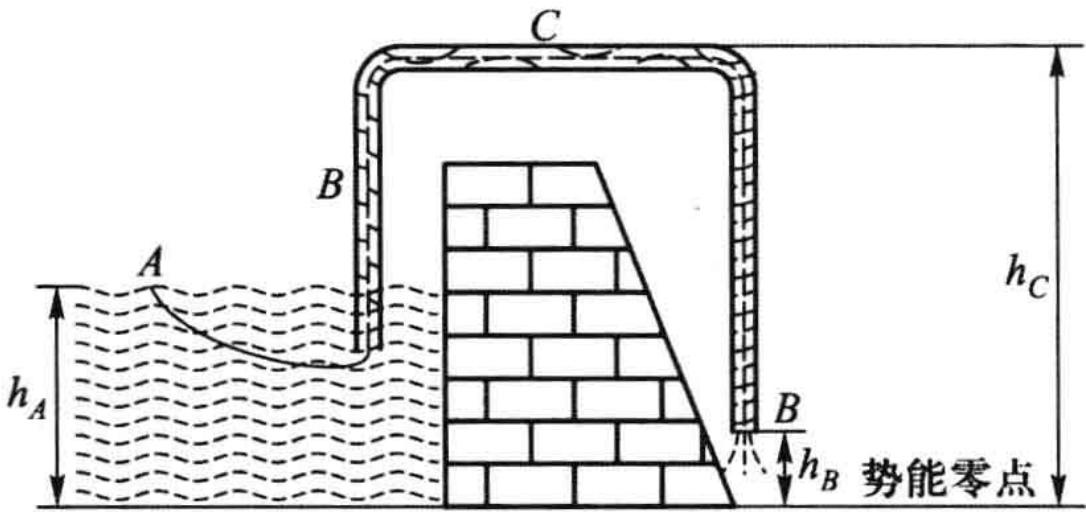
\includegraphics[width=0.4\textwidth]{figures/fig8-7.jpg}
  \end{figure}

\vfill

\textbf{8-8.}如习题 8-8 图所示,一水平管下面装有一 U 形管,U 形管内盛有水银。已知水平管中粗、细处的横截面积分别为, $S_{A}=5.0 \times 10^{-3} \mathrm{~m}^{2}, S_{B}=1.0 \times 10^{-3} \mathrm{~m}^{2}$ 。当水平管中有水流做定常流动时,测得 U 形管中水银面的高度差为 $h=3.0 \times 10^{-2} \mathrm{~m}$ 。求水流在粗管处的流速 $v$ 。已知水和水银的密度分别为 $\rho=1.0 \times 10^{3} \mathrm{~kg/m}^{3}, \rho'=13.6 \times 10^{3} \mathrm{~kg/m}^{3}$ 。

\begin{figure}[H]
  \centering
  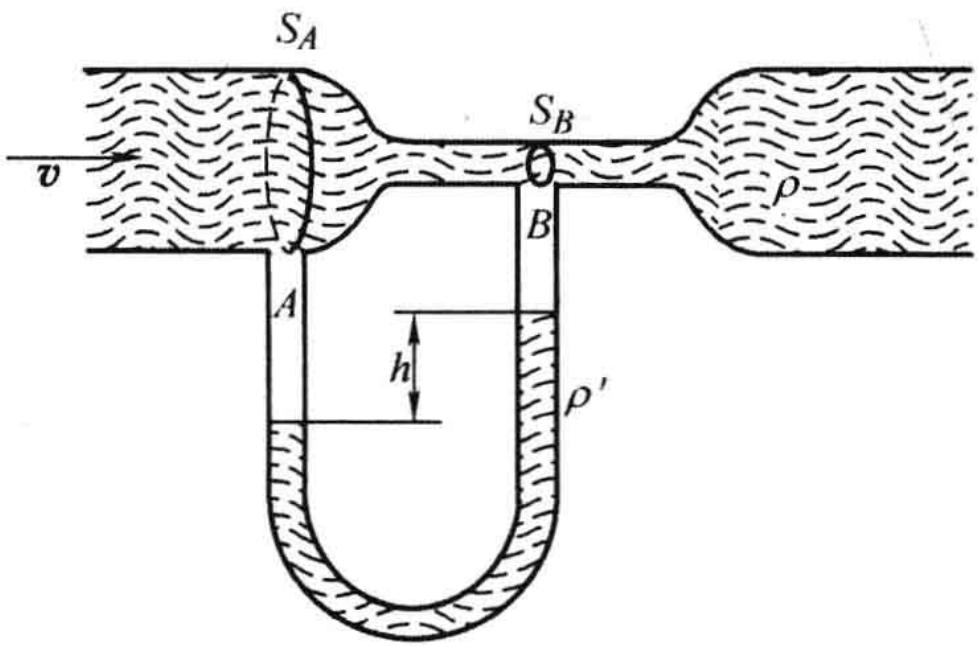
\includegraphics[width=0.4\textwidth]{figures/fig8-8.jpg}
  \end{figure}

\vfill
\newpage

\textbf{8-9.}利用压缩空气把水从一密封的容器内通过一管子压出,如习题 8-9 图所示。已知管子的出口处比容器内水面高 $h = 0.50 \mathrm{~m}$ 。当水从管口以 $1.5 \mathrm{~m} / \mathrm{s}$ 的流速流出时，求容器内空气的压强。

\begin{figure}[H]
  \centering
  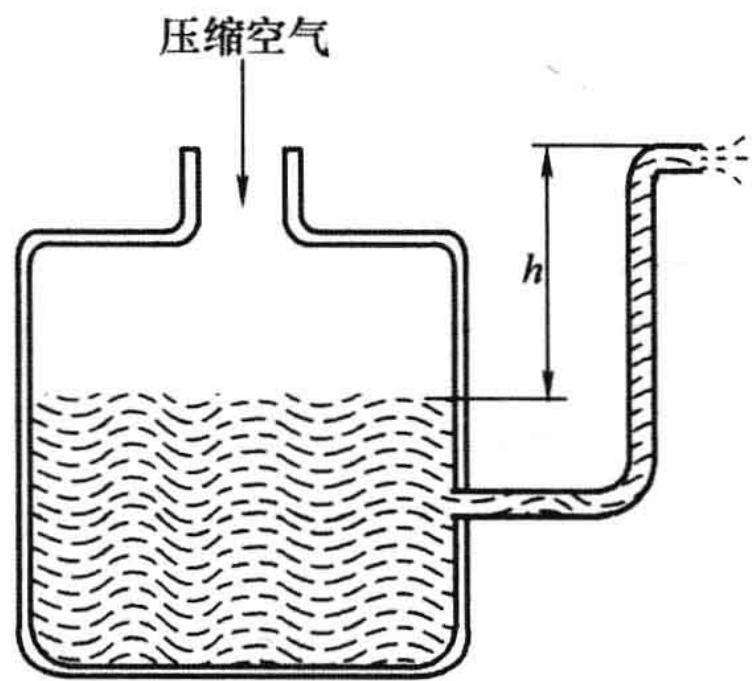
\includegraphics[width=0.35\textwidth]{figures/fig8-9.jpg}
  \end{figure}

\vfill

\textbf{8-10.}一喷泉竖直喷出高度为 $H$ 的水流, 喷泉的喷嘴具有上细下粗的截锥形状。上截面的直径为 $d_{1}$ , 下截面的直径为 $d_{2}$ , 喷嘴高为 $h$ 。设大气压强为 $p_{0}$ , 求:

(1) 水的体积流量；

(2) 喷嘴下截面处的压强。

\vfill
\newpage

\textbf{8-11.}如习题 8-11 图所示, 在一大容器的底部接一竖直管, 在 $B$ 处装有一压力计竖直管的下口 $C$ 处用软木塞塞住。若 $A$ （容器内液面处）、$B$ 、$C$ 三点的高度分别为 $h_A,h_B,h_C$ 。求:

(1) 此时压力计中液面的高度 $h_{1}$ ;

(2) 拔去软木塞, 当水做定常流动后, 压力计中液面的高度 $h_{2}$ 。

\begin{figure}[H]
  \centering
  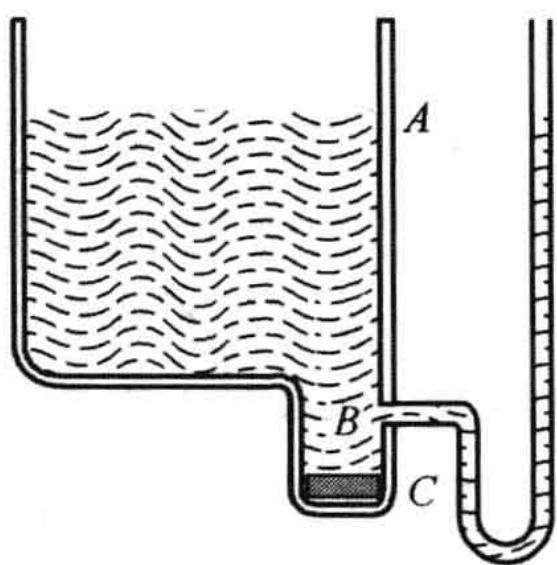
\includegraphics[width=0.25\textwidth]{figures/fig8-11.jpg}
  \end{figure}

\vfill

\textbf{8-12.}在一截锥形容器内盛有高度为 $h = 0.7 \mathrm{~m}$ 的水, 其侧壁与底面成 $\theta = 60^{\circ}$ 角, 容器被放在高为 $h_0 = 0.50 \mathrm{~m}$ 的物体上, 在容器壁的底部开有一小孔, 如习题 8-12 图所示。求水从小孔射出后的水平射程 $L$ 。

\begin{figure}[H]
  \centering
  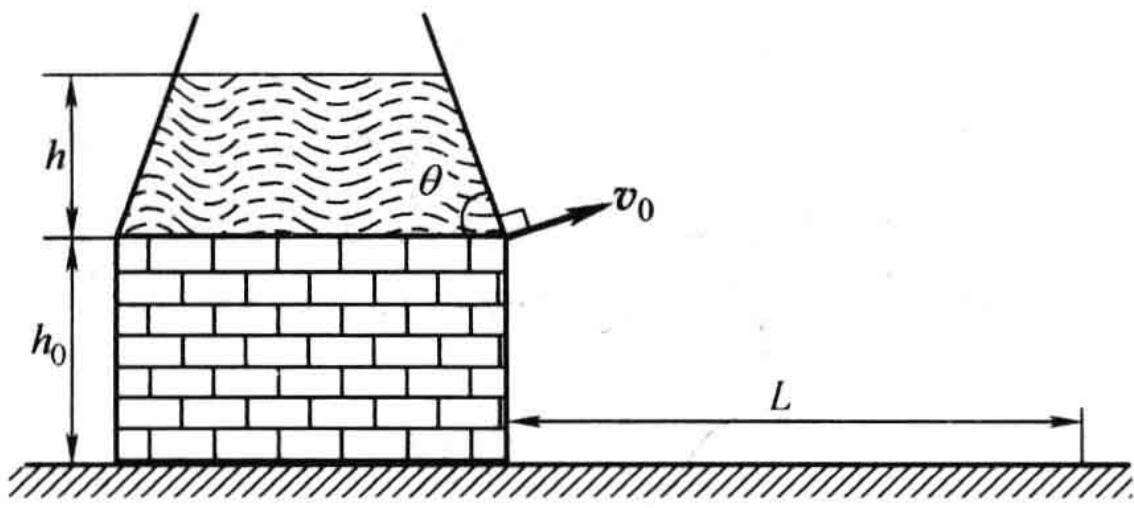
\includegraphics[width=0.35\textwidth]{figures/fig8-12.jpg}
  \end{figure}

\vfill
\newpage


\textbf{8-13.}在某水池的边上装有一宽为 $1.0 \mathrm{~m}$ , 高为 $2.0 \mathrm{~m}$ 的小门, 其下边与水池底相平, 并用铰链与池壁连接。试问, 当池内的水深刚好没过门时, 门受到的水的作用力相对于铰链的力矩为多大?

\begin{figure}[H]
  \centering
  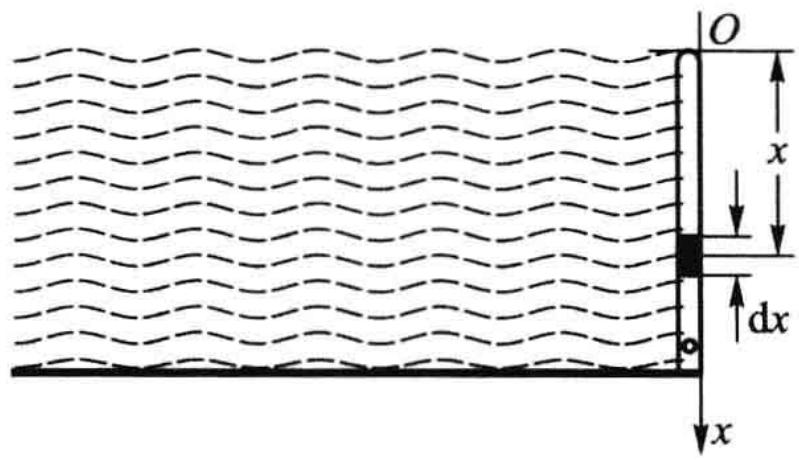
\includegraphics[width=0.35\textwidth]{figures/fig8-13.jpg}
  \end{figure}

\vfill

\textbf{8-14.}在一直径很大的圆柱形水桶壁的近底部处有一个直径为 $0.04 \mathrm{~m}$ 的小孔。若桶内水的深度为 $1.60 \mathrm{~m}$ 。

(1) 求此时水从小孔中流出的体积流量 $Q_{1}$ 。

(2) 若小孔为薄壁圆孔, 其收缩系数为 $61\%$ 。求实际的体积流量 $Q_{2}$ , 并求由于收缩现象的存在而造成的计算值与实际值之间的百分误差。

\vfill
\newpage

\textbf{8-15.}液体在一水平管道中流动, $A$ 处和 $B$ 处的横截面积分别为 $S_A$ 和 $S_B$ , $B$ 管口与大气相通, 压强为 $p_0$ , 若在 $A$ 处用一细管与容器相通, 如习题 8-15 图所示, 试证明: 当 $h$ 满足下式 $h = \frac{Q^2}{2g}\left(\frac{1}{S_A^2} - \frac{1}{S_B^2}\right)$ 时, $A$ 处的压强刚好能将比水平管低 $h$ 处的同种液体吸上来。其中 $Q$ 为体积流量。

\begin{figure}[H]
  \centering
  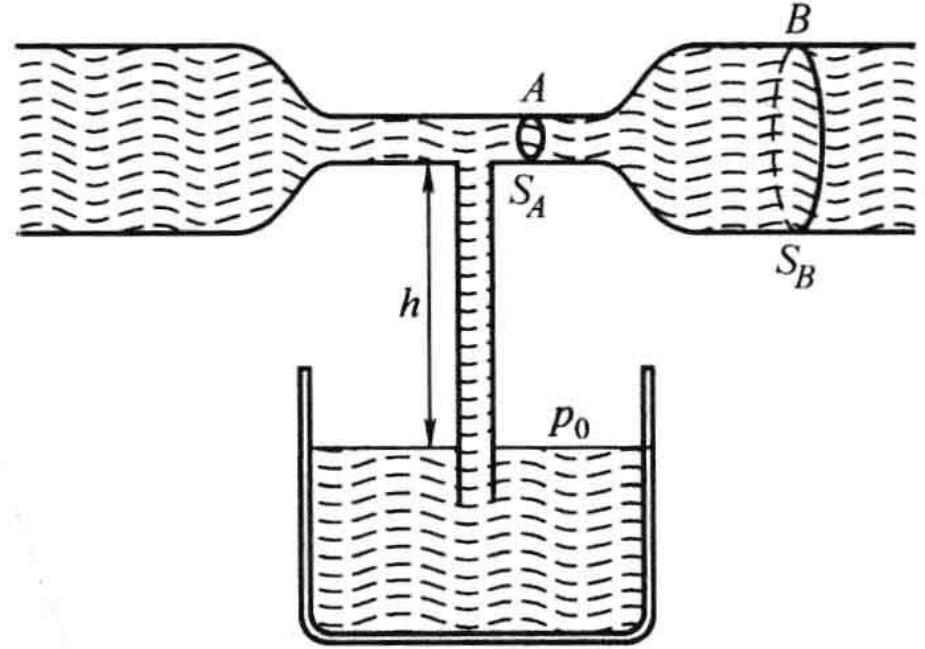
\includegraphics[width=0.25\textwidth]{figures/fig8-15.jpg}
  \end{figure}

\vfill

\textbf{8-16.}在一大容器的底部有一小孔, 容器横截面积与小孔面积之比为 100, 容器内盛有高度 $h = 0.80 \mathrm{~m}$ 的水。求容器内水流完所需的时间。设在整个过程中, 水的流动可视为定常流动。

\vfill
\newpage

\textbf{8-17.}一根长为 $L$ 的水平粗管与一根竖直细管连接成如习题8-17图所示的形状。把细管的下端插入密度为 $\rho_{\mathrm{f}}$ 的液体中，然后将粗管的管口封住，并使其绕细管以恒定的角速度 $\omega$ （很小）旋转，如习题8-17图所示。已知粗管在绕轴旋转之前，其内空气的密度为 $\rho_{\mathrm{a}}$ ，压强为$p_{a}$ 。设细管的体积与粗管相比可以忽略,忽略毛细现象和旋转前后管内空气密度的变化。求细管中液体上升的高度 h 。设温度不变。

\begin{figure}[H]
  \centering
  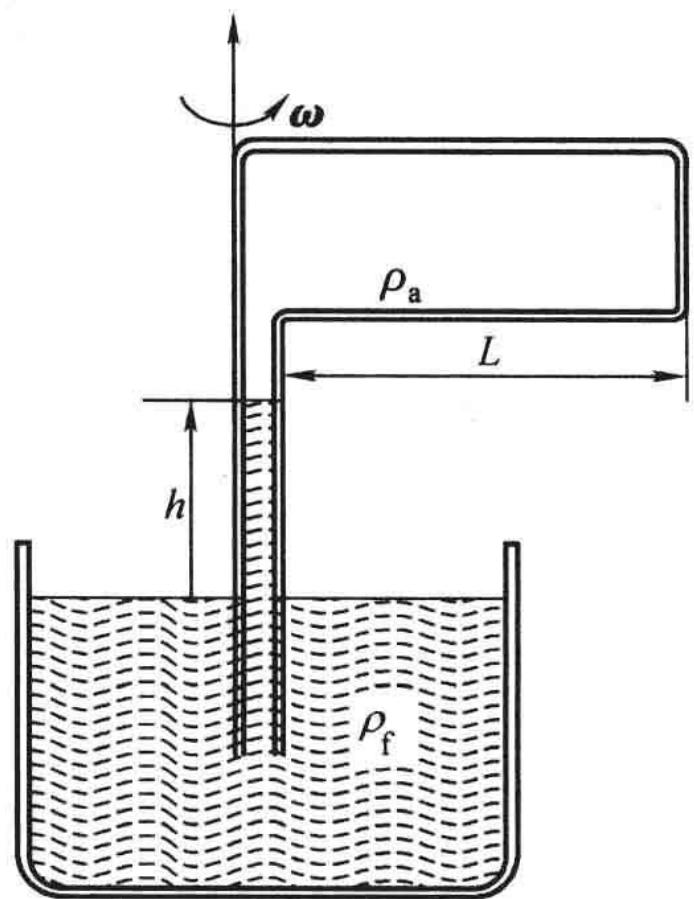
\includegraphics[width=0.25\textwidth]{figures/fig8-17.jpg}
  \end{figure}

\vfill

\textbf{8-18.}一个半径 $r = 0.20 \times 10^{-2} \mathrm{~m}$ 的小球落入 $\rho = 0.90 \times 10^{3} \mathrm{~kg} / \mathrm{m}^{3}$ 的黏性液体中。已知小球的密度 $\rho' = 6.5 \times 10^{3} \mathrm{~kg} / \mathrm{m}^{3}$ , 并测得小球在该液体中的最终速度 $v_{\mathrm{f}} = 0.24 \mathrm{~m} / \mathrm{s}$ 。试求:

(1) 液体的黏度 $\eta$ ;

(2) 小球在下降过程中加速度为 $\frac{1}{3} g$ 时刻的速度 $v$ 。


\vfill
\newpage